\documentclass[12pt]{article}
\usepackage{mathptmx}
\usepackage{fullpage}
\usepackage{multicol}
\usepackage{amsmath,amssymb}
\usepackage[aux]{rerunfilecheck}
\usepackage{tikz}
\usepackage{wrapfig}

\newcommand{\ds}{\displaystyle}

\reversemarginpar

\usepackage{lastpage,fancyhdr}
\usepackage{fancyhdr}
\pagestyle{fancy}
\lhead{MATH110 200930 Quiz 9      \\
  Time: 20 minutes                        \\ \quad }
\chead{Page\ \thepage\ of \pageref{LastPage}   \\ \quad \\ \quad}
\rhead{Name: \underline{\hspace{1.5in}}        \\
  Student \#: \underline{\hspace{1.5in}}  \\ \quad }
\cfoot{}
\addtolength{\headheight}{\baselineskip}
\addtolength{\headheight}{\baselineskip}
\addtolength{\headheight}{\baselineskip}
\addtolength{\headheight}{\baselineskip}
\renewcommand{\headrulewidth}{0pt}
\fancypagestyle{plain}{%
  \lhead{}
  \chead{FIRST NATIONS UNIVERSITY OF CANADA             \\
    DEPARTMENT OF SCIENCE \\
    MATH110 200930 Quiz 9 \\
    \quad                                      }
  \rhead{}
  \cfoot{Page\ \thepage\ of \pageref{LastPage}}
}

\begin{document}
\thispagestyle{plain}

\begin{flushleft}
Time:  20 minutes                \hfill       Name: \underline{\hspace{2in}} \\
Instructor: Dr. Edward Doolittle \hfill Student \#: \underline{\hspace{2in}}
\end{flushleft}

\noindent
Please\marginpar{\centering (marks)} do questions 1 and 2.  You have 10 minutes to do each question, for a total of 20
minutes for the quiz.  A %non-programmable
calculator of the type mentioned in the course outline is allowed.
%but is not necessary.  
%You may leave early if you can
%do so without disturbing any of your colleagues.
%If you finish early, I suggest you check your work thoroughly.
%\textbf{Please do not disturb your colleagues by climbing over them while
%they are trying to write the quiz.}

\begin{enumerate}
\item A\marginpar{\centering (10)}
  Norman window has the shape of a rectangle surmounted by a semicircle.
  If the perimeter of the window must be 40 meters, find the dimensions of
  the window with greatest area.  Hint: the area of a semicircle of radius
  $r$ is $\pi r^2/2$, and the perimeter of the curved part of the 
  semicircle is $\pi r$.
  \\
  %\begin{wrapfigure}{r}{3cm}
  %\centering
  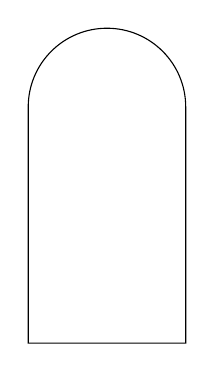
\begin{tikzpicture}
    \draw (0,0) -- (2,0) -- (2,3) arc (0:180:1) -- cycle;
  \end{tikzpicture}
  %\end{wrapfigure}
\vfill
\newpage
\item Find\marginpar{\centering (10)} 
  $\ds s(t)$ given that $\ds s''(t)=60t^4-24t^2+2$, $\ds s(0)=-1$, $\ds s'(0)=5$.
\end{enumerate}

\end{document}

